\documentclass{elsart}

\journal{Science of Computer Programming}

% Packages.tex

% Packages di latex utilizzati 

  % Standard dell'ams
\usepackage{amssymb,amsmath}

  % Per le definizioni di connessioni di Galois
\usepackage{galois}

  % Per formattare ed includere il testo
\usepackage{lgrind}
     % Cambiamento dei font per lgrind: tutti in Courier
\def\CMfont{\ttfamily\itshape}
\def\KWfont{\ttfamily\bfseries}
\def\VRfont{\ttfamily}
\def\BGfont{\ttfamily}
\def\NOfont{\ttfamily}

  % Caratteri speciali per i nomi di funzione
\usepackage{bbm}

  % Caratteri ``cal'' carini
\usepackage[mathcal]{euscript}

  % per \baro
\usepackage{stmaryrd}

  % per \xspace
\usepackage{xspace}

  % per i diagrammi
\usepackage[all]{xy}

  % for scalebox
\usepackage{graphicx}
 
   % Per le figure incastrate l'una nell'altra
\usepackage{subfigure}

  % Per le figure nel testo
\usepackage{wrapfig}


\usepackage{tabularx}

  % Per includere i verbatim
\newbox\subfigbox
\makeatletter
\newenvironment{subfloat}
{\def\caption##1{\gdef\subcapsave{\relax##1}}%
\let\subcapsave\@empty
\setbox\subfigbox\hbox
\bgroup}
{\egroup
\subfigure[\subcapsave]{\box\subfigbox}}
\makeatother

   % Per la compilazione Condizionale
\usepackage{ifthen}

\usepackage{empheq}

   % Per i riferimenti incrociati



%\ifx\pdfoutput\undefined % Se compilo con ``latex'' ed uso ps2pdf
%\usepackage{color}
%\usepackage[dvips]{graphicx}       %%% graphics for dvips
%\DeclareGraphicsExtensions{.eps}   %%% standard extension for included graphics
%\usepackage[bookmarks=true]{hyperref}
%\else                    % Se compilo con ``pdflatex'' 
%\usepackage[pdftex]{graphicx}      %%% graphics for pdfLaTeX 
%\DeclareGraphicsExtensions{.pdf}   %%% standard extension for included graphics
%\usepackage[pdftex]{thumbpdf}      %%% thumbnails for pdflatex
%\usepackage[pdftex,                %%% hyper-references for pdflatex
%bookmarks=true,%                   %%% generate bookmarks ...
%bookmarksnumbered=true,%           %%% ... with numbers
%hypertexnames=false,%              %%% needed for correct links to figures !!!
%breaklinks=true,%                  %%% break links if exceeding a single line
%linkbordercolor={0 0 1}]{hyperref} %%% blue frames around links
%                                  %%% pdfborder={0 0 1} is the default
%\hypersetup{
%pdfauthor   = {Francesco Logozzo \& Agostino Cortesi},
%pdftitle    = {to be decided},
%pdfsubject  = {Objects},
%pdfkeywords = {Abstract Interpretation, Static Analysis, Object Oriented}
%}
%\pdfadjustspacing=1                %%% force LaTeX-like character spacing
%\fi 


%%% Local Variables: 
%%% mode: plain-tex
%%% TeX-master: "main"
%%% End: 

% Definizione dei simboli

\newcommand{\eg}{\textit{e.g.}}
\newcommand{\ie}{\textit{i.e.}}

% Definizione dell' operatore di astrazione
\newcommand{\abs}[1]{\ensuremath{\bar{\mathsf{#1}}}}

\newcommand{\sx}{\llbracket}
\newcommand{\dx}{\rrbracket}

  % Semantica generica
\newcommand{\sem}[1]{\ensuremath{\sx \mathtt{#1} \dx}}

  % Semantica che prende un nome
\newcommand{\semantica}[2]{\ensuremath{\mathbb{#1}\sem{#2}}}

\newcommand{\BigSemantica}[2]{\ensuremath{\mathbb{#1}{\Bigg\llbracket #2 \Bigg\rrbracket}}}

  % Semantiche generiche
\newcommand{\csem}[1]{\ensuremath{\semantica{s}{#1}}}
\newcommand{\asem}[1]{\ensuremath{\semantica{\abs{s}}{#1}}}
\newcommand{\asemRefined}[1]{\ensuremath{\semantica{\abs{s}^*}{#1}}}

  % Funzione di ``transfer''
\newcommand{\trasf}[1]{\ensuremath{\semantica{t}{#1}}}
\newcommand{\atrasf}[1]{\ensuremath{\semantica{\abs{t}}{#1}}}

  % Semantica di: costruttore,  metodo
\newcommand{\semcostr}[1]{\semantica{i}{#1}}
\newcommand{\semmetodo}[1]{\semantica{m}{#1}}
\newcommand{\semoggetto}[1]{\semantica{o}{#1}}
\newcommand{\semclasse}[1]{\semantica{c}{#1}}

  % Semantica Colleting Traces
\newcommand{\Semmetodo}[1]{\semantica{M}{#1}}
\newcommand{\Semoggetto}[1]{\semantica{O}{#1}}
\newcommand{\Semclasse}[1]{\semantica{C}{#1}}

  % Semantics Reachable States
\newcommand{\rsemcostr}[1]{\semantica{I}{#1}}
\newcommand{\rsemmetodo}[1]{\Semmetodo{#1}}
\newcommand{\rsemoggetto}[1]{\semantica{O}{#1}}
\newcommand{\rsemclasse}[1]{\semantica{C}{#1}}

  % Seamntica Astratta
\newcommand{\asemcostr}[1]{\semantica{\bar{I}}{#1}}
\newcommand{\asemmetodo}[1]{\semantica{\bar{M}}{#1}}
\newcommand{\asemoggetto}[1]{\semantica{\bar{O}}{#1}}
\newcommand{\asemclasse}[1]{\semantica{\bar{C}}{#1}}

  % Operazioni su stati
\newcommand{\less}{\ensuremath{\sqsubseteq}}
\newcommand{\join}{\ensuremath{\sqcup}}
\newcommand{\meet}{\ensuremath{\sqcap}}
\newcommand{\bottom}{\ensuremath{\bot}}
\newcommand{\bigjoin}{\ensuremath{\bigsqcup}}

  % Semantica astratta
\newcommand{\asemantica}[2]{\semantica{\bar{#1}}{#2}}
\newcommand{\asemanticaBig}[2]{\BigSemantica{\bar{#1}}{#2}}


  % Semantica astratta BIS, per aggiungere pedici
\newcommand{\asemanticaBis}[3]{\semantica{\bar{#1}_{\textit{#2}}}{#3}}

  % Operazioni astratte
\newcommand{\nabs}[1]{\bar{#1}}
\newcommand{\abot}{\nabs{\bot}}
\newcommand{\atp}{\nabs{\ensuremath{\top}}}
\newcommand{\aless}{\nabs{\less}}
\newcommand{\asup}{\ensuremath{\nabs{\sqsupseteq}}}
\newcommand{\acup}{\ensuremath{\nabs{\sqcup}}}
\newcommand{\ajoin}{\acup}
\newcommand{\abigcup}[1]{\nabs{\bigsqcup_{#1}}}
\newcommand{\abigjoin}[1]{\abigcup{#1}}
\newcommand{\acap}{\ensuremath{\nabs{\sqcap}}}
\newcommand{\ameet}{\acap}
\newcommand{\abigcap}[1]{\nabs{\bigsqcap_{#1}}}
\newcommand{\abigmeet}[1]{\abigcap{#1}}


 % lfp : least fixpoint
\newcommand{\lfp}[2]{\ensuremath{\mathrm{lfp}^{#1}_{#2}}}

 % gfp: greatest fixpoint
\newcommand{\gfp}[2]{\ensuremath{\mathrm{gfp}^{#1}_{#2}}}


% Insiemi e Funzioni

  % Insieme, elemento di insieme, nessun elemento
\newcommand{\insieme}[1]{\ensuremath{\mathsf{#1}}}
\newcommand{\el}[1]{\ensuremath{\mathsf{#1}}}
\newcommand{\noel}{\el{\bot}}

  % Insieme delle parti
\newcommand{\parti}[1]{\ensuremath{\mathcal{P}{(#1)}}}
\newcommand{\partiFin}[1]{\ensuremath{\mathcal{P}_{\mathrm{fin}}{(#1)}}}


  % Elementi di insiemi
\newcommand{\noval}{\ensuremath{\baro}}

  % Cardinalita di inisiemi
\newcommand{\cardinalita}[1]{\ensuremath{\# #1}}

  % Env, Store, Addr, Val, Label : Scorciatoie
\newcommand{\env}{\insieme{Env}}
\newcommand{\Env}{\env}

\newcommand{\aenv}{\ensuremath{\bar{\env}}}

\newcommand{\store}{\insieme{Store}}
\newcommand{\Store}{\store}

\newcommand{\astore}{\ensuremath{\overline{\store}}}

\newcommand{\AState}{\abs{\Sigma}}
\newcommand{\astate}{\AState}

\newcommand{\addr}{\insieme{Addr}}
\newcommand{\Addr}{\addr}

\newcommand{\aaddr}{\ensuremath{\overline{\addr}}}

\newcommand{\Reference}{\insieme{Ref}}
\newcommand{\reference}{\reference}

\newcommand{\AReference}{\ensuremath{\overline{\Reference}}}

\newcommand{\val}{\insieme{Val}}

\newcommand{\etichetta}{\insieme{Label}}
\newcommand{\cont}{\ensuremath{\kappa}}

  % Stati
\newcommand{\stati}[1]{\ensuremath{\Sigma}}
  % Tracce
\newcommand{\tracce}[1]{\ensuremath{\mathcal{T}(#1)}}
  % Transizione
\newcommand{\tr}[1]{\ensuremath{\xrightarrow{#1}}}

  % Insieme di funzioni
\newcommand{\funzione}[2]{\ensuremath{[#1 \rightarrow#2]}}

  % Funzione vuota
\newcommand{\emptyfun}{\ensuremath{[\cdot]}}

  % Insieme di funzioni monotone e joim-morphism
\newcommand{\funmon}[2]{\ensuremath{[#1 \stackrel{m}{\longrightarrow} #2]}}
\newcommand{\funjoin}[2]{\ensuremath{[#1 \stackrel{\sqcap}{\longrightarrow} #2]}}

% Astratto
  % Dominio concreto
\newcommand{\dom}[1]{\insieme{#1}}

  % Dominio astratto
\newcommand{\adom}[1]{\ensuremath{{\mathsf{#1}}}}

 % Vari domini
\newcommand{\Intervals}{\dom{Intv}}
\newcommand{\LT}{\dom{LT}}
\newcommand{\Boxes}{\dom{Boxes}}
\newcommand{\DBM}{\dom{DBM}}
\newcommand{\Octagons}{\dom{Oct}}
\newcommand{\Polyhedra}{\dom{Poly}}
\newcommand{\Poly}{\Polyhedra}
\newcommand{\Lineq}{\dom{LinEq}}
\newcommand{\LinEq}{\Lineq}
\newcommand{\Karr}{\Lineq}
\newcommand{\Symbolic}{\dom{Symb}}
\newcommand{\Pentagons}{\dom{Pnt}}
\newcommand{\SubPolyhedra}{\dom{SubPoly}}
\newcommand{\SubPoly}{\SubPolyhedra}
\newcommand{\Subpoly}{\SubPolyhedra}

  % Elemento di dominio astratto
\newcommand{\ael}[1]{\ensuremath{\abs{\el{#1}}}}
\newcommand{\aelBis}[2]{\ensuremath{\abs{\el{#1}}_\el{#2}}}

  % Funzione di astrazione e concretizzazione
\newcommand{\alfa}{\ensuremath{\alpha}}
%\renewcommand{\gamma}{\ensuremath{\gamma}}
\newcommand{\gm}{\ensuremath{\gamma}}


% Funzioni usate nella tesi
  % Transizione basica
\newcommand{\prossimo}{\ensuremath{\mathrm{next}}}
%\newcommand{\next}{\ensuremath{\mathrm{next}}}
\newcommand{\nextDir}{\ensuremath{\mathrm{next_{dir}}}}
\newcommand{\nextInd}{\ensuremath{\mathrm{next_{ind}}}}
\newcommand{\prossimoDir}{\nextDir}
\newcommand{\prossimoInd}{\nextInd}

  % Transizione ``collecting''
\newcommand{\Next}{\ensuremath{\mathrm{Next}}}
\newcommand{\NextDir}{\ensuremath{\mathrm{Next_{dir}}}}
\newcommand{\NextInd}{\ensuremath{\mathrm{Next_{ind}}}}

  % Reachable addresses
\newcommand{\reachable}{\ensuremath{\mathrm{reachable}}}
  % Update function
\newcommand{\update}{\ensuremath{\mathrm{update}}}
  % Storia delle interazioni
%\newcommand{\etichette}{\ensuremath{\mathrm{labels}}}
\newcommand{\storia}{\ensuremath{\mathrm{history}}}

  % Contesto
\newcommand{\contesto}{\ensuremath{\mathrm{Context}}}

  % Contesto Astratto
\newcommand{\acontesto}{\ensuremath{\mathrm{\overline{Context}}}}

% Tracce : definizioni
\newcommand{\stringavuota}{\ensuremath{\epsilon}}


% Funzioni di astrazione
  % Prima Astrazione, quella dei metodi
\newcommand{\alfaPrima}{\ensuremath{\alpha_{\Yright}}}
\newcommand{\gammaPrima}{\ensuremath{\gamma_{\Yright}}}
  % Versione higher-order
\newcommand{\alfaPrimaDot}{\ensuremath{\dot{\alpha}_{\Yright}}}

  % Seconda Astrazione, quella degli stati
\newcommand{\alfaSeconda}{\ensuremath{\alpha_{\circ}}}
\newcommand{\gammaSeconda}{\ensuremath{\gamma_{\circ}}}
  % Versione higher-order
\newcommand{\alfaSecondaDot}{\ensuremath{\dot{\alpha}_{\circ}}}


\newcommand{\alfaAddr}{\ensuremath{\alpha_\el{a}}}
\newcommand{\gammaAddr}{\ensuremath{\gamma_\el{a}}}

\newcommand{\gammaBool}{\ensuremath{\gamma_\el{b}}}

\newcommand{\gammaEnv}{\ensuremath{\gamma_\el{e}}}

\newcommand{\gammaOct}{\ensuremath{\gamma_\el{o}}}
\newcommand{\gammaDOct}{\ensuremath{\gamma_\el{do}}}

\newcommand{\gammaRef}{\ensuremath{\gamma_\el{r}}}

\newcommand{\gammaStore}{\ensuremath{\gamma_\el{s}}}

\newcommand{\gammaState}{\ensuremath{\gamma_{\astate}}}

% Estensioni per OO

  % Classe
\newcommand{\classe}[1]{\ensuremath{\mathtt{#1}}}
\newcommand{\classi}{\ensuremath{\mathcal{C}}}

  % Gerarchia
\newcommand{\gerarchia}[1]{\ensuremath{\mathcal{#1}}}
\newcommand{\gerarchie}{\ensuremath{\mathbb{H}}}

  % Operatori su Gerarchie 
\newcommand{\inserisciClasse}{\ensuremath{\uplus}}
\newcommand{\costruisciClasse}{\ensuremath{\beta}}
\newcommand{\unisciGerarchie}{\ensuremath{\Cup}}

\newcommand{\aclasse}[1]{\ensuremath{\abs{\mathtt{#1}}}}
\newcommand{\aclasseLong}[1]{\ensuremath{\overline{\mathtt{#1}}}}
  % Oggetto, instanza di classe
\newcommand{\oggetto}[1]{\ensuremath{\mathsf{#1}}}
  % Metodo
\newcommand{\metodo}[1]{\ensuremath{\mathtt{#1}}}
  % Campo
\newcommand{\campo}[1]{\ensuremath{\mathtt{#1}}}

  % Astrazioni di campi
\newcommand{\acampo}[1]{\ensuremath{\mathtt{\abs{#1}}}}

  % Astrazione di metodi con constraints
\newcommand{\ametodo}[1]{\ensuremath{\mathtt{\abs{#1}}}}

% Dominio delle Tracce Collecting

\newcommand{\adomTracce}{\ensuremath{\adom{D}_{\Yright}}}

\newcommand{\atopTracce}{\ensuremath{\abs{\top}_{\Yright}}}
\newcommand{\abottomTracce}{\ensuremath{\abs{\bot}_{\Yright}}}

\newcommand{\alessTracce}{\ensuremath{\abs{\subseteq}_{\Yright}}}
\newcommand{\alessTraccia}{\ensuremath{\abs{\subseteq}^{\tau}_{\Yright}}}

\newcommand{\ajoinTracce}{\ensuremath{\abs{\cup}_{\Yright}}}
\newcommand{\ajoinTraccia}{\ensuremath{\abs{\cup}^{\tau}_{\Yright}}}

\newcommand{\ameetTracce}{\ensuremath{\abs{\cap}_{\Yright}}}
\newcommand{\ameetTraccia}{\ensuremath{\abs{\cap}^{\tau}_{\Yright}}}

% Scorciatoie

  % ``Prende''
\newcommand{\prende}{\ensuremath{\mapsto}}

  % Simbolo di definizione
\newcommand{\df}{\ensuremath{\triangleq}}

  % Tupla
\newcommand{\tupla}[1]{\ensuremath{\langle #1 \rangle}}

  % Stati Iniziali
\newcommand{\statiiniziali}[1]{\ensuremath{S_0\tupla{#1}}}

  % Modularita
\newcommand{\hasA}{has-A}
\newcommand{\isA}{is-A}

  % Riferimento ad una formula
\newcommand{\formula}[1]{\ensuremath{\mathrm{(\ref{#1})}}}

% Complessita

  % O-notation
\newcommand{\costo}[1]{\ensuremath{\kappa_{#1}}}


% Definizioni per i domini di vincoli

\newcommand{\Vars}{\ensuremath{\mathtt{Vars}}}
\newcommand{\C}{\ensuremath{\dom{C}}}
\newcommand{\initC}{\ensuremath{\mathrm{initial_{\C}}}}

\newcommand{\dominio}{\ensuremath{\mathrm{dom}}}
\newcommand{\range}{\ensuremath{\mathrm{range}}}

  % Relazioni
\newcommand{\rel}[1]{\ensuremath{\mathsf{\rho}[\mathtt{#1}]}}
\newcommand{\conDuepar}[2]{\ensuremath{\con'[\mathtt{#1}, \mathtt{#2}]}}
\newcommand{\conTrepar}[3]{\ensuremath{\con[\mathtt{#1}, \allowbreak \mathtt{#2}, \allowbreak \mathtt{#3}]}}
\newcommand{\relass}[1]{\ensuremath{\rho(#1)}}

\newcommand{\rgamma}{\ensuremath{\gamma_{\rho}}}
\newcommand{\cgamma}{\ensuremath{\gamma_{\C}}}

 % Lettera
\newcommand{\con}{\ensuremath{\mathsf{c}}}

 % Sequenza
\newcommand{\seq}[1]{\ensuremath{\vartriangleright_\mathtt{#1}}}


 % Semantiche per i vincoli
\newcommand{\semc}[1]{\semantica{s}{#1}}

\newcommand{\semtracce}[1]{\semantica{t}{#1}}
\newcommand{\asemtracce}[1]{\semantica{\bar{t}}{#1}}
\newcommand{\asemtracces}[1]{\semantica{\bar{s}}{#1}}


\newcommand{\modsem}[1]{\ensuremath{\semantica{T}{#1}}}
\newcommand{\amodsem}[1]{\semantica{\bar{T}}{#1}}

\newcommand{\A}{\ensuremath{\adom{A}}\xspace}
\newcommand{\modA}{\ensuremath{\adom{A}_\mathsf{M}}\xspace}
\newcommand{\Absel}{\ensuremath{\ael{a}}\xspace}
\newcommand{\modAbsel}{\ensuremath{\ael{a}_\mathsf{m}}\xspace}

\newcommand{\relsem}[1]{\semantica{R}{#1}}

 % Proiezione/dropping

\newcommand{\lascia}{\ensuremath{\delta}}
\newcommand{\tieni}{\ensuremath{\pi}}

%\newcommand{\Absless}{\ensuremath{\sqsubseteq^\mathsf{a}}}
\newcommand{\modAbsless}{\ensuremath{\abs{\sqsubseteq}_\mathsf{m}}}

%\newcommand{\Absjoin}{\ensuremath{\sqcap^\mathsf{a}}}
\newcommand{\modAbsjoin}{\ensuremath{\abs{\sqcap}_\mathsf{m}}}

\newcommand{\aconc}{\ensuremath{\abs{\odot}}\xspace}


 % Operazioni sul dominio di vincoli
\newcommand{\cless}{\ensuremath{\preceq}}
\newcommand{\cgreater}{\ensuremath{\succeq}}
\newcommand{\ctop}{\ensuremath{\vernal}}
\newcommand{\cbot}{\ensuremath{\bot^\con}}
\newcommand{\cmeet}{\ensuremath{\curlywedge}}
\newcommand{\cjoin}{\ensuremath{\curlyvee}}
\newcommand{\cwiden}{\ensuremath{\hbox{\hbox to 0pt{\raisebox{4pt}{$\relbar$}}$\curlyvee$}}}
\newcommand{\bigcjoin}{\ensuremath{\bigcurlyvee}}

\newcommand{\alg}{\ensuremath{\mathcal{A}}}

 % Definizione di BodyOf
\newcommand{\bodyof}[1]{\ensuremath{\mathrm{bodyOf}(\mathbf{#1})}}

 % Definitione di tiedVars
\newcommand{\tiedvars}{\ensuremath{\mathrm{tiedVars}}}

  % Operazioni su Tracce
%\newcommand{\tracce}[1]{\ensuremath{\wp(#1^\infty)}\xspace}
\newcommand{\iniziatracce}[2]{\ensuremath{\mathcal{T}(#1,#2)}}
\newcommand{\giunzione}{\ensuremath{\frown}\xspace}
\newcommand{\conc}{\ensuremath{\odot}\xspace}
\newcommand{\last}{\ensuremath{\mathrm{last}}}

  % Funzioni Semantiche ``Astratte''
\newcommand{\flow}[1]{\ensuremath{\mathrm{flow}_\mathtt{#1}}}
\newcommand{\aflow}[1]{\ensuremath{\overline{\mathrm{flow}}_\mathtt{#1}}}

  % Definizione di ``approssima'', i.e. un vincolo approssima la semantica di un metodo
\newcommand{\approssima}{\ensuremath{\Subset}}

  % Approssimazione con vincoli della semantica di un metodo
\newcommand{\conmetodo}[5]{\ensuremath{\con_{#1}[\mathtt{#2}, \allowbreak \mathtt{#3}, \allowbreak \mathtt{#4}, \allowbreak \mathtt{#5}]}}



% Definizione del dominio degli osservabili
\newcommand{\osservabile}[2]{\ensuremath{\mathcal{O}_{#2}(\classe{#1})}}
\newcommand{\oless}{\ensuremath{{\sqsubseteq}_{o}}}
\newcommand{\osup}{\ensuremath{{\sqsupseteq}_{o}}}
\newcommand{\ojoin}{\ensuremath{{\sqcup}_{o}}}
\newcommand{\omeet}{\ensuremath{{\sqcap}_{o}}}
\newcommand{\otp}{\ensuremath{{\top}_{o}}}
\newcommand{\obot}{\ensuremath{{\bot}_{o}}}
\newcommand{\obigjoin}{{{\bigsqcup}{}}_{o}}

\newcommand{\domPiuPreciso}{\ensuremath{O[\parti{\Sigma}]}}

% Interfaccia di una classe
\newcommand{\interfaccia}[1]{\ensuremath{\iota(\classe{#1})}}


% Definizione dell' insieme delle astrazioni di un dominio +
% operazioni

\newcommand{\astrazioni}[1]{\ensuremath{\mathcal{A}(#1)}}
\newcommand{\dless}{\ensuremath{\leq}}
\newcommand{\djoin}{\ensuremath{\vee}}
\newcommand{\dmeet}{\ensuremath{\wedge}}

% Dominio dei valori
\newcommand{\dominioVal}[1]{\ensuremath{\mathit{#1}}}

% Stato interno ad un oggetto
\newcommand{\stato}{\ensuremath{\sigma}}

% Semantica backward concreta ed astratta
\newcommand{\backSemmetodo}[1]{\semantica{{M}^{<}}{#1}}
\newcommand{\abacksemmetodo}[1]{\semantica{\bar{M}^{<}}{#1}}


% Complexity
\newcommand{\Order}[1]{\ensuremath{\mathcal{O}(#1)}}

% Keywords

\newcommand{\Clousot}{\ensuremath{\mathtt{Clousot}}}

\newcommand{\code}[1]{\ensuremath{\mathtt{#1}}}

\newcommand{\takes}{\ensuremath{\leftarrow}}

\newcommand{\linea}[1]{\ensuremath{#1}}



% Syntax

\newcommand{\Assert}{\ensuremath{\mathtt{assert}}~}
\newcommand{\Assume}{\ensuremath{\mathtt{assume}}~}
\newcommand{\While}{\code{while}}
\newcommand{\If}{\code{if}}
\newcommand{\Else}{\code{else}}
\newcommand{\Skip}{\code{skip}}

\newcommand{\Stm}{\code{Stm}}
\newcommand{\Var}{\code{Var}}
\newcommand{\Exp}{\code{Exp}}
\newcommand{\BExp}{\code{BExp}}
\newcommand{\Bexp}{\BExp}
\newcommand{\ExpTwoOps}{\code{ExpTwoOps}}
\newcommand{\Lit}{\code{Lit}}
\newcommand{\Op}{\code{op}}
\newcommand{\Relop}{\code{relop}}
\newcommand{\Int}{\code{int}}

\newcommand{\Code}{\code{IstrStream}}
\newcommand{\Label}{\code{Label}}
\newcommand{\Istr}{\code{Istr}}
\newcommand{\Jump}{\code{jmp}}
\newcommand{\JumpIfTrue}{\code{jmpIf}}
\newcommand{\JumpIf}{\JumpIfTrue}
\newcommand{\Nop}{\code{nop}}

\newcommand{\Comp}{\ensuremath{\mathcal{C}}}
\newcommand{\Compexp}{\ensuremath{\mathcal{C}_{e}}}
\newcommand{\CompExp}{\Compexp}

\newcommand{\assign}{\el{assign}}
\newcommand{\test}{\el{test}}
\newcommand{\guard}{\test}
\newcommand{\checkif}{\el{check}}
\newcommand{\checkIf}{\checkif}

\newcommand{\aassign}{\el{\assign}}
\newcommand{\atest}{\el{\test}}

\newcommand{\arange}{\el{\mathsf{range}}}

\newcommand{\widening}{\ensuremath{\triangledown}}
\newcommand{\awidening}{\widening}
\newcommand{\narrowing}{\ensuremath{\vartriangle}}

\newcommand{\HLsem}[1]{\asemantica{H}{#1}}
\newcommand{\HLSem}[1]{\HLsem{#1}}
\newcommand{\LLsem}[1]{\asemantica{L}{#1}}
\newcommand{\LLSem}[1]{\LLsem{#1}}

\newcommand{\BigLLSem}[1]{\asemanticaBig{L}{#1}}
\newcommand{\bigLLSem}[1]{\BigLLSem{#1}}
\newcommand{\bigLLsem}[1]{\BigLLSem{#1}}

\newcommand{\result}{\code{res}}

% Definizioni per Subpolyhedra


\newcommand{\VarProg}{\ensuremath{\Var_\mathtt{P}}}
\newcommand{\VarSlack}{\ensuremath{\Var_\mathtt{S}}}

\newcommand{\variable}[1]{\ensuremath{\mathtt{#1}}}

\newcommand{\var}{\variable{v}}

\newcommand{\progvar}{\variable{x}}
\newcommand{\progvariable}[1]{\ensuremath{\progvar_{#1}}}

\newcommand{\slackvariable}[1]{\ensuremath{\beta_{#1}}}
\newcommand{\slackvar}{\slackvariable{}}

\newcommand{\slackvariableinfo}[1]{\ensuremath{\code{info}(#1)}}
\newcommand{\slackvarinfo}{\slackvariableinfo{\slackvariable{}}}


\newcommand{\reduction}[1]{\ensuremath{\rho(#1)}}
\newcommand{\simplify}[1]{\ensuremath{\sigma(#1)}}

\newcommand{\bottomS}{\ensuremath{\bottom_{S}}}
\newcommand{\topS}{\ensuremath{\top_{S}}}
\newcommand{\lessS}{\ensuremath{\aless_{S}}}
\newcommand{\joinS}{\ensuremath{\join_{S}}}
\newcommand{\wideningS}{\ensuremath{\widening_{S}}}

\newcommand{\intv}{\ael{i}}
\newcommand{\lineq}{\ael{l}}

\newcommand{\subpoly}{\ael{s}}

\newcommand{\subpolyPair}[2]{\ensuremath{\tupla{\lineq_{#1}^{#2};\ \intv_{#1}^{#2}}}}

%% Subsection trick to save some vertical space
\newcommand{\Fsubsubsection}[1]{\smallskip\noindent\textbf{#1}}


\newcommand{\Foxtrot}{\code{Foxtrot}}
\newcommand{\NET}{\code{.Net}}


\newcommand{\hint}[1]{\ensuremath{\mathbbm{h}_{#1}}}
\newcommand{\op}{\ensuremath{\diamond}}

\newcommand{\hintcomp}{\ensuremath{\Xi}}

\begin{document}

\begin{frontmatter}

\title{Pentagons: A Weakly Relational Abstract Domain for the Efficient Validation of Array Accesses}

\author{Francesco Logozzo}
\address{Microsoft Research, Redmond, WA, USA}
\ead{logozzo@microsoft.com}

\author{Manuel F\"ahndrich}
\address{Microsoft Research, Redmond, WA, USA}
\ead{maf@microsoft.com}


\begin{abstract}
We introduce Pentagons (\Pentagons),  a weakly relational numerical abstract
domain useful for the validation of array accesses in byte-code and
intermediate languages (IL).
This abstract domain captures properties of the form of $\code{x} \in [a, b] \wedge \code{x} < \code{y}$.
It is more precise than the well known Interval
domain, but it is less precise than the Octagon domain.

The goal of \Pentagons{} is to be a lightweight numerical domain useful
for adaptive static analysis, where \Pentagons{} 
is used to quickly prove the safety of most array accesses, restricting the use of
more precise (but also more expensive) domains to only a small fraction of the code.

We implemented the \Pentagons{} abstract domain in \Clousot, a generic
abstract interpreter for .NET assemblies. Using it, we were able to
validate $83\%$ of array accesses in the core runtime library
\code{mscorlib.dll} in a little bit more than 3 minutes.
\end{abstract}


\begin{keyword}
Abstract Domains \sep Abstract Interpretation \sep Bounds checking \sep Numerical Domains \sep Static Analysis \sep .NET Framework
\end{keyword}

\end{frontmatter}

\section{Introduction}
The goal of an abstract interpretation-based static analysis is to
statically infer properties of the execution of a program that can be
used to ascertain the absence of certain runtime failures.
Traditionally, such tools focus on proving the absence of out of bound memory accesses, 
divisions by zero, overflows, or null dereferences.

The heart of an abstract interpreter is the abstract domain, which captures the properties of interest for the analysis.
In particular,  several \emph{numerical} abstract domains have been
developed, \eg,~\cite{CousotHalbwachs78,Mine01-2,SimonKing02}, that
are useful to check properties such as out of bounds and division by zero, but also aliasing \cite{Venet02}, parametric predicate abstraction \cite{Cousot03} and resource usage ~\cite{Navas07}.

In this paper we present  Pentagons, \Pentagons, a new numerical
abstract domain designed and implemented as part of \Clousot{}, a generic static analyzer based on abstract interpretation of MSIL~\cite{MSIL}.
We intend \Clousot{} to be used by developers during coding and
testing phases. It should therefore be scalable, yet sufficiently precise.
To achieve this aim, \Clousot{} is designed to adaptively choose the
necessary precision of the abstract domain, as opposed to fixing it
\emph{before} the analysis (\eg, \cite{Logozzo07}).
Thus, \Clousot{} must be able to discharge most of the ``easy checks''
very quickly, hence focusing the analysis only on those pieces of code
that require a more precise abstract domain or fixpoint strategy.

\Clousot{} uses the abstract domain of \Pentagons{} to quickly analyze .NET assemblies and discharge most of the proof obligations from the successive phases of the analysis.
As an example let us consider the code in Figure~\ref{fig:exBinSearch}, taken from the basic component library of .NET.
\Clousot{}, instantiated with the abstract domain \Pentagons,
automatically discovers  the following invariant at program point $\mathtt{(*)}$:
\[ 
0 \leq \code{num} < \code{array.Length} \wedge 0 \leq \code{num2} < \code{array.Length}
\]
This is sufficient to prove that $0 \leq \code{index} < \code{array.Length}$, \ie, the array is never accessed outside of its bounds.

The elements of \Pentagons{} are of the form $\code{x} \in [a, b]\wedge \code{x} < \code{y}$, where $\code{x}$ and $\code{y}$ are program variables and $a, b$ are rationals.
Such elements allow expressing (most)  bounds of program variables,
and in particular those of array indices: intervals $[a,b]$ take care of the numerical part (\eg, to check array  underflows $0 \leq a$), and inequalities $\code{x} < \code {y}$ handle the symbolic reasoning (\eg, to check array overflows $\code{x} < \code{arr.Length}$).

\Pentagons{} is therefore an abstract domain more precise than the
Intervals, \Intervals ~\cite{CousotCousot77}, as it adds
symbolic reasoning, but it is less precise than Octagons, \Octagons
~\cite{Mine01-2}, as it cannot for instance capture equalities such as $\code{x} + \code{y} == 22$. 
We found that \Pentagons{} is precise enough to validate $83\%$ of
the array bound accesses (lower and upper) in \code{mscorlib.dll}, the main library in the .NET platform, in less than 4 minutes.
Similar results are obtained for the other assemblies of the .NET framework.
Thus,  \Pentagons{}  fits well with the programming style adopted in this library.
Nevertheless, it is not the ultimate abstract domain for bounds analysis. 
For instance, when used on part of \Clousot's implementation, it
validates only $72\%$ of the accesses. 



\newcommand\codefamily\sffamily
\lstset{language={[Sharp]C},mathescape=false,flexiblecolumns=true,morekeywords={},basicstyle=\codefamily\small,frame=lines,moredelim=[is][\itshape]{@}{@},captionpos=b,numberstyle=\tiny,stepnumber=1,numbersep=2pt}

\begin{figure}[t]
\begin{lstlisting}[language={[Sharp]C}]
    int BinarySearch(ulong[] array, ulong value)
    {
      int num = 0;
      int num2 = array.Length - 1;
      while (num <= num2)
      { (*)
        int index = (num + num2) >> 1;
        ulong num4 = array[index];
        if (value == num4)
          return index;
        if (num4 < value)       
          num = index + 1;        
        else       
          num2 = index - 1;        
      }
      return ~num;
    }
\end{lstlisting}
\vspace*{-2mm}
\caption{Example from \code{mscorlib.dll}. \Pentagons{} infers the loop
  invariant $0 \leq  \code{num} \wedge \code{num2} <
  \code{array.Length}$  which is enough to prove that $0 \leq
  \code{index} <  \code{array.Length}$ holds at array access.}
\label{fig:exBinSearch}
\end{figure}



\section{Basics of Abstract interpretation}

Abstract interpretation is a theory of approximations, \cite{CousotCousot77}.
It captures the intuition that semantics are more or less precise depending on the observation level.
The observation level is formalized by the notion of an abstract domain.
An abstract domain \adom{D} is a complete lattice
\tupla{\el{E},\aless, \abot, \atp, \acup, \acap}, where \el{E} is the
set of abstract elements, ordered according to relation $\aless$.  
The smallest abstract element is $\abot$, the largest is $\atp$. 
The join \acup, and the meet \acap,  are also defined.
When the abstract domain \adom{D} does not respect the ascending chain
condition, then a widening operator \awidening{} must be used to
enforce the termination of the analysis. 
With a slight abuse of notation, sometimes we will confuse an
abstract domain \adom{D} with the set of its elements \el{E}. 


A  domain \adom{D} is the abstraction of a concrete domain
\dom{C} = \tupla{\el{C},\ \cless,\ \abot,\ \atp, \cjoin, \cmeet}, if it
exists a pair of monotonic functions (Galois connection)
$\tupla{\alpha, \gamma}$ such that: (i) $\alpha \in 
\funzione{\dom{C}}{\adom{D}}$ (abstraction); (ii) $\gamma \in
\funzione{\adom{D}}{\dom{C}}$ (concretization); and (iii) $\forall \el{c} \in
\dom{C}. \forall \el{d} \in \adom{D}.\ \alpha(\el{c}) \aless \el{d}
\Leftrightarrow \el{c} \cless \gamma(\el{d})$ (soundness).
In a Galois connection, one adjoint determines the
other~\cite{CousotCousot77}, and in particular the concretization
function uniquely defines the abstraction: 
$\alpha = \lambda \el{c}.\ \meet \{ \el{d} \mid \el{c} \cless
\gamma(\el{d}) \}$, so that often we will omit of the two.



The \emph{best} abstract transfer
function for a concrete transfer function $\mathsf{t} \in
\funzione{\dom{C}}{\dom{C}}$, is   $\mathsf{t^a_*} = \alpha \circ \mathsf{t} \circ
\gamma$~\cite{CousotCousot77}.
In general, the best abstract transfer function is not computable, and
a sound approximation $\mathsf{t^a}$, such that  $\forall \ael{d} \in
\adom{D}.\ \mathsf{t^a_*}(\ael{d}) \less \mathsf{t^a}(\ael{d})$, is
often good enough.

Given a concrete domain \dom{C} and two domains $\adom{D}_1$ and
$\adom{D}_2$, related to \dom{C} respectively by two Galois connections
$\tupla{\alpha_1, \gamma_1}$ and $\tupla{\alpha_2, \gamma_2}$, then
the relation $\equiv$ defined as $\tupla{d_1, d_2} \equiv \tupla{d'_1,
  d'_2}$ iff $\gamma_1(d_1) \cmeet \gamma_2(d_2) =  \gamma_1(d'_1)
\cmeet \gamma_2(d'_2)$ is an equivalence relation.
The quotient domain $(\adom{D}_1 \times \adom{D}_2)_{/\equiv}$ is 
the \emph{reduced} Cartesian product of $\adom{D}_1$ and $\adom{D}_2$.
We let $\adom{D}_1 \otimes \adom{D}_2$ denote the reduced product of
two abstract domains.

\section{Numerical Abstract Domains}

A \emph{numerical} abstract domain \adom{N} is an abstract domain
which approximates sets of numerical values, \eg, one such
concretization is  $\gamma \in \funzione{\adom{N}}{\parti{\Sigma}}$, where
$\Sigma = \funzione{\code{Vars}}{\mathbb{Z}}$ is an environment,
mapping variables to integers.

When designing numerical abstract domains, one wants to fine tune the
cost-precision ratio.  Consider the points in Figure~\ref{fig:concrete}.
They represent the concrete values that two variables, \code{index} and \code{a.Length},
can take at a given program point for \emph{all} possible
executions.  As there may be many such values or an unbounded number
of them, computing this set precisely is either too expensive or
infeasible. Abstract domains over-approximate such sets and thereby
make them tractable.

\begin{figure*}[t]
\centering
\subfigure[Concrete points]
{
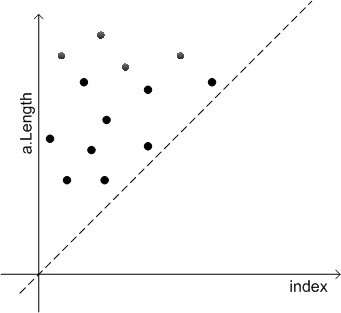
\includegraphics[scale=.4]{Original.png}
\label{fig:concrete}
}
\qquad
\subfigure[Intervals]
{
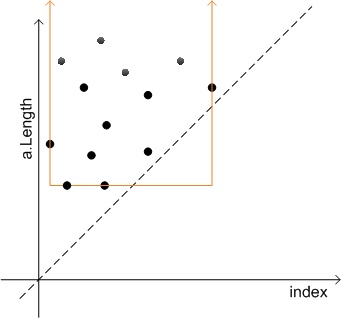
\includegraphics[scale=.4]{Intervals.png}
\label{fig:intervals}
}

\smallskip

\subfigure[Octagons]
{
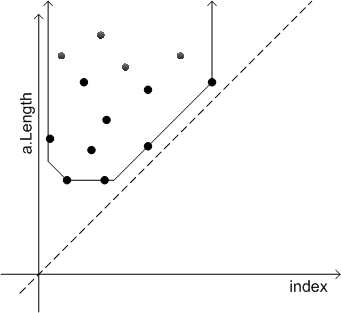
\includegraphics[scale=.4]{Octagons.png}
\label{fig:octagons}
}
\qquad
\subfigure[Pentagons]
{
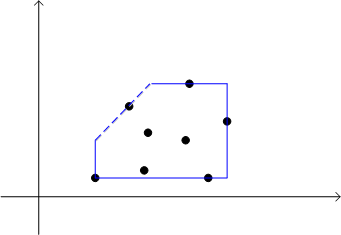
\includegraphics[scale=.4]{Pentagons.png}
\label{fig:pentagons}
}
\caption{The concrete points, and some approximations depending on the numerical abstract domain}
\label{fig:example}
\end{figure*}

\subsection{Intervals} 
A first abstraction of the points in Fig~\ref{fig:concrete} can be
made by retaining only the minimum and maximum values of variables \code{index} and \code{a.Length}.
This is called interval abstraction. Graphically, it boils down to enveloping the concrete values with a rectangle, as depicted in Figure~\ref{fig:intervals}.
The abstract domain of intervals is very cheap, as it requires
storing only two integers for each variable, and all the operations can be performed in linear time (w.r.t. the number of variables).
However, it is also quite imprecise, in particular because it cannot capture relations between variables.
For instance, in Figure~\ref{fig:intervals} the fact that $\code{index} < \code{a.Length}$ is lost.
 

\subsection{Octagons}
A more precise abstraction is obtained by using the abstract domain of Octagons, \Octagons. 
\Octagons{} keeps relations of the form $\pm \code{x} \pm \code{y} \leq k$.
When applied to our concrete points, the octagon enveloping them is shown in Figure~\ref{fig:octagons}.
\Octagons{} can capture relations between two variables---desirable
when analyzing array bounds---but its complexity is $\Order{n^2}$ in space and $\Order{n^3}$ in time.
The cubic complexity is a consequence of the closure algorithm used by all the domain operations.
Bagnara \emph{et al.} gave a precise bound for it in \cite{Bagnara05}. The standard closure operator on \Octagons{} performs $20 n^3 + 24  n^2$ coefficient operations, that can be reduced to $16n^3 + 4n^2 +4n$ with a smarter algorithm.

While having polynomial complexity, \Octagons{} unfortunately does not
scale if many variables are kept in the same octagon.
For this reason the technique of buckets has been independently introduced in  \cite{BlanchetCousotEtAl03} and \cite{Venet04}.
The intuition behind it is to create many octagons, each relating few variables, \eg,  no more than $4$.
The problem with this technique is how to choose the bucketing of
variables. Existing heuristics use the structure of the source program.

\subsection{Pentagons}
The approximation of the concrete points with \Pentagons{} is given in Figure~\ref{fig:pentagons}.
Elements of \Pentagons{} have the form of $\code{x} \in [a, b] \wedge \code{x} < \code{y}$, where $\code{x}$ and $\code{y}$ are variables and $a$ and $b$ belong to some underlying numerical set as $\mathbb{Z}$ or $\mathbb{Q}$, extended with $-\infty$ and $+\infty$.
A pentagon keeps lower and upper bounds for each variable, so it is as precise as intervals, but it also keeps strict inequalities among variables so that it enables a (limited) form of symbolic reasoning.
It is worth noting that the region of the plane that is delimited by a (two dimensional) pentagon may not be closed.
In fact, if the underlying numerical values are in $\mathbb{Q}$, then $\code{x} < \code{y}$ denotes an open surface of $\mathbb{Q}^2$, whereas if they are in $\mathbb{Z}$, then $\code{x} < \code{y}$ is equivalent to $\code{x} \leq \code{y} -1$, which is a closed region of $\mathbb{Z}^2$.

We found pentagons quite efficient in practice. 
The complexity is $\Order{n^2}$, both in time and space.
Furthermore, in our implementation we perform the expensive operation
(the closure) either lazily or in an incomplete (but sound) way, so
that the domain shows an almost linear behavior in practice.

\section{Interval Environments}
The elements of the abstract domain of intervals, \Intervals, are $\{ [i, s] \mid i,s \in \mathbb{Z} \cup \{-\infty, + \infty\} \}$.
The formal definition of the lattice operations on intervals is recalled in Figure~\ref{tab:intervals}.
The order is the interval inclusion, the bottom  element is the empty
interval (\ie, an interval where $s < i$), the largest element is the
line $[-\infty, +\infty]$, the join and the meet are respectively the
convex hull and the intersection of intervals.
The widening preserves the bounds which are stable. 

The concretization function, $\gamma_\Intervals \in \funzione{\Intervals}{\parti{\mathbb{Z}}}$ is defined as $\gamma_\Intervals([i, s]) = \{ z \in \mathbb{Z} \mid i \leq z \leq s\}$.

\begin{figure}
\small
\begin{tabular}{rl}
Order:& $[a_1, b_1] \iless [a_2, b_2] \Longleftrightarrow a_1 \geq a_2 \wedge b_1 \leq b_2$ \\
Bottom:& $ [a, b] = \ibot \Longleftrightarrow a > b$ \\
Top:& $[a, b] = \itop \Longleftrightarrow a = -\infty \wedge b = +\infty$\\
Join:& $[a_1, b_1] \ijoin [a_2, b_2] = [\mathrm{min}(a_1, a_2), \mathrm{max}(b_1, b_2)]$ \\
Meet:& $[a_1, b_1] \imeet [a_2, b_2] = [\mathrm{max}(a_1, a_2), \mathrm{min}(b_1, b_2)]$ \\
Widening:& $[a_1, b_1] \iwidening [a_2, b_2] = [a_1 \leq a_2 ? a_2 : -\infty, b_1 \geq b_2 ? b_2 : +\infty]$ \\
\end{tabular}
\caption{Lattice operations over single intervals}
\label{tab:intervals}
\end{figure}

The abstract domain of interval environments, \Boxes, is the functional lifting of \Intervals, \ie, $\Boxes =  \funzione{\Vars}{\Intervals}$.
The lattice operations are hence the functional extension of those in Figure~\ref{tab:intervals}, as shown by Figure~\ref{tab:boxes}.

The concretization of a box, $\gamma_\Boxes \in \funzione{\Boxes}{\parti{\Sigma}}$ is defined as $\gamma_\Boxes(f) = \{ \sigma \in \Sigma \mid \forall \code{x}. \code{x} \in f \Longrightarrow \sigma(\code{x}) \in \gamma_\Intervals(f(\code{x}))\}$.

The assignments and the guards in the interval environment are defined as usual in interval arithmetic~\cite{Cousot98}.

\begin{figure}
\small
\begin{tabular}{rl}
Order:& $ b_1 \bless b_2 \Longleftrightarrow \forall \code{x} \in b_1. b_1(\code{x}) \iless b_2(\code{x})$ \\
Bottom:& $ b = \bbot \Longleftrightarrow \exists \code{x} \in b. b(\code{x}) = \ibot$ \\
Top:& $ b = \btop \Longleftrightarrow \forall \code{x} \in b. b(\code{x}) = \itop$\\
Join:& $ b_1 \bjoin b_2 = \lambda \code{x}. b_1(\code{x}) \ijoin b_2(\code{x}) $ \\
Meet:& $ b_1 \bmeet b_2 = \lambda \code{x}. b_1(\code{x}) \imeet b_2(\code{x}) $  \\
Widening:&  $b_1 \bwidening b_2 = \lambda \code{x}. b_1(\code{x}) \iwidening b_2(\code{x}) $
\end{tabular}
\caption{Lattice operations of interval environments}
\label{tab:boxes}
\end{figure}
 

\section{Strict upper bounds}
The abstract domain of strict upper bounds \SUB{} is a special case of
the zone abstract domains ~\cite{Mine02,GaubertEtAl07}, which keeps symbolic information in the form of $\code{x} < \code{y}$.
We represent elements of \SUB{} with maps $\code{x} \mapsto \{ \code{y}_1, \dots \code{y}_n \}$ with the meaning that \code{x} is strictly smaller than each of the $\code{y}_i$.
Maps enable very efficient implementations.
The formal definition of the lattice operations for \SUB{} is in Figure~\ref{tab:sub}.

\begin{figure}
\small
\begin{tabular}{rl}
Order:& $ s_1 \sless s_2 \Longleftrightarrow \forall \code{x} \in s_2. s_1(\code{x}) \supseteq s_2(\code{x})$ \\
Bottom:& $ s = \sbot \Longleftrightarrow  \exists \code{x,y} \in s. \code{y} \in s(\code{x}) \wedge \code{x} \in s(\code{y})$ \\
Top:& $ s = \sTop \Longleftrightarrow \forall \code{x} \in s. s(\code{x}) = \emptyset$\\
Join:& $ s_1 \sjoin s_2 = \lambda \code{x}. s_1(\code{x}) \cap s_2(\code{x}) $ \\
Meet:& $ s_1 \smeet s_2 = \lambda \code{x}. s_1(\code{x}) \cup s_2(\code{x}) $  \\
Widening:&  $s_1 \swidening s_2 = \lambda \code{x}. s_1(\code{x}) \subseteq s_2(\code{x}) ? s_2(\code{x}) : \emptyset $
\end{tabular}
\caption{Lattice operations of strict upper bounds}
\label{tab:sub}
\end{figure}
\hyphenation{pre-sent}
Roughly, the fewer constraints the less information is  present.
As a consequence, the order is given by the (pointwise) superset inclusion, the bottom environment is one which contains a contradiction $\code{x} < \code{y} \wedge \code{y} < \code{x}$ and the lack of information, \ie, the top element is represented by the empty set.
The join is (pointwise) set intersection: at a join point we want to keep those relations that hold on both (incoming) branches.
The meet is (pointwise) set union: relations that hold on either the left \emph{or} the right branch.
Finally, widening is defined in the usual way: we keep those
constraints that are stable in successive iterations.

The concretization function, $\gamma_\SUB \in \funzione{\SUB}{\parti{\Sigma}}$ is defined as $\gamma_\SUB(s) = \cap_{\code{x} \in s} \{ \sigma \in \Sigma \mid \code{y} \in s(\code{x}) \Longrightarrow \sigma(\code{x}) < \sigma(\code{y}) \}$.



We deliberately skipped the discussion of the closure operation until now.
One may expect to endow the \SUB{} abstract domain with a
saturation rule for transitivity such as
\[
\frac{\code{y} \in s(\code{x}) \quad \code{z} \in s(\code{y})}{\code{z} \in s(\code{x})}
\]
and apply it to the abstract values prior to applying the join in
Figure~\ref{tab:sub}, thereby inferring and retaining the maximum possible constraints.
However it turns out that the systematic application of the saturation
rule requires $\Order{n^3}$ operations, which voids the efficiency
advantage of \Pentagons.
In \Clousot, we chose to not perform the closure, and instead improved
the precision of individual transfer functions.
 They infer new relations $\code{x} < \code{y}$ and use a limited transitivity driven by the program under analysis. 
So, for instance:
\[
\begin{array}{rcl}
\sem{x := y - 1}(s) & = & s[\code{x} \mapsto \{ \code{y}\} \cup s(\code{y})], \text{if \code{x} does not appear in}\ s \\ 
\sem{x == y}(s) & = & s[\code{x}, \code{y} \mapsto s(\code{x}) \cup s(\code{y})] \\
\sem{x < y}(s) &=& s[\code{x} \mapsto s(\code{x}) \cup s(\code{y}) \cup \{ \code{y}\}] \\
\sem{x \leq y}(s) &=& s[\code{x} \mapsto s(\code{x}) \cup s(\code{y})]  
\end{array}
\]
because we know that (i) if we subtract a positive constant from a
variable we obtain a result strictly smaller \footnote{In this paper
  we ignore overflows. However our abstract semantics of arithmetic
  expressions in \Clousot{} takes care of them.}, that (ii) when we
compare two variables for equality they must satisfy the same
constraints, and that (iii) for each $\code{z}$ such that $\code{y} <
\code{z}$, if  $\code{x} < \code{y}$ or $\code{x} \leq \code{y}$ then
$\code{x} < \code{z}$. 

\section{Pentagons}
A first approach to combine the numerical properties captured by
\Intervals, and the symbolic ones captured by \SUB{} is to consider
the Cartesian product  $\Intervals \times \SUB$. 
Such an approach is equivalent to running the two analyses in
parallel, without any exchange of information between the two
domains. 
A better solution is to perform the \emph{reduced} Cartesian product
$\Intervals \otimes \SUB$. 
Roughly, the reduced Cartesian product of a product lattice smashes together
the pairs that have the same concrete meaning.
The \Pentagons{} abstract domain is an abstraction of the reduced
product and is more precise than the Cartesian product. 


The lattice operations are defined in Figure~\ref{tab:pentagons}.
The functions $\mathrm{sup}$ and $\mathrm{inf}$ are defined as  $\mathrm{inf}([a,b]) = a$ and $\mathrm{sup}([a,b]) = b$.

The order on \Pentagons{} is a refined version of the pairwise order: a pentagon $\tupla{b_1, s_1}$ is smaller than a pentagon $\tupla{b_2, s_2}$ iff the interval environment $b_1$ is included in $b_2$ and for all the symbolic constraints $\code{x} < \code{y}$ in $s_2$, either $\code{x} < \code{y}$ is an explicit constraint in $s_1$ or it is implied by the interval environment $b_1$, \ie, the numerical upper bound for \code{x} is strictly smaller than the numerical lower bound for \code{y}.

A pentagon is bottom if either its numerical component \emph{or} the symbolic component are.
A pentagon is top if both the numerical component \emph{and} the symbolic component are.

For the numerical part, the join operator pushes the join to the underlying \Intervals{} abstract domain, and for the symbolic part, it keeps the constraints which are either explicit in the two operators \emph{or} which are explicit in one operator, and implied by the numerical domain in the other component. 
We will further discuss the join, cardinal for the scalability and the precision of the analysis below.

The meet and the widening operators simply delegate the meet and the widening to the underlying abstract domains.
Note that we do not perform any closure before widening in order to
avoid well known convergence problems arising from the combination of widening and closure operations~\cite{Mine01-2}.

\begin{figure}
\small
\begin{tabular}{rl}
Order:& $\tupla{b_1, s_1} \pless \tupla{b_2, s_2}   \Longleftrightarrow  b_1 \bless b_2 $ \\
& $ \qquad \quad \wedge (\forall \code{x} \in s_2 \forall\code{y} \in s_2(\code{x}). \code{y} \in s_1(\code{x}) \vee\ \mathrm{sup}(b_1(\code{x})) < \mathrm{inf}(b_1(\code{y}))) $ \\
Bottom:& $\tupla{b, s}  = \pbot \Rightarrow b = \bbot \vee  s = \sbot $ \\
Top:& $ \tupla{b, s} = \ptop \Longleftrightarrow b = \btop \wedge s = \sTop $\\
Join:& $\tupla{b_1, s_1}  \pjoin  \tupla{b_2, s_2}  = $ \\
& $\quad \mathrm{let}\ b^\sqcup = b_1 \bjoin b_2$ \\
& $\quad \mathrm{let}\ s^\sqcup = \lambda \code{x}.  s'(\code{x}) \cup s''(\code{x}) \cup s'''(\code{x})$ \\
& $\quad \quad \mathrm{where}\ s' = \lambda \code{x}. s_1(\code{x}) \cap s_2(\code{x})$ \\
& $\quad \phantom{\lambda \code{x}.} \mathrm{and}\ s'' = \lambda \code{x}. \{\code{y} \in s_1(\code{x}) \mid \mathrm{sup}(b_2(\code{x})) < \mathrm{inf}(b_2(\code{y})) \}$ \\
& $\quad  \phantom{\lambda \code{x}.} \mathrm{and}\ s''' =  \lambda \code{x}. \{\code{y} \in s_2(\code{x}) \mid \mathrm{sup}(b_1(\code{x})) < \mathrm{inf}(b_1(\code{y})) \}$ \\
& $\quad \mathrm{in}\ \tupla{ b^\sqcup, s^\sqcup}$ \\
Meet:& $ \tupla{b_1, s_1}  \pmeet  \tupla{b_2, s_2}  = \tupla{b_1 \bmeet b_2, s_1 \smeet s_2} $  \\
Widening:&  $ \tupla{b_1, s_1}  \pwidening \tupla{b_2, s_2}  = \tupla{b_1 \bwidening b_2, s_1 \swidening s_2}$
\end{tabular}
\caption{The lattice operations over Pentagons}
\label{tab:pentagons}
\end{figure} 


\subsection{Cost and Precision of the Join}
One may ask why we defined the join over \Pentagons{} as in Figure~\ref{tab:pentagons}.
In particular, a more natural definition may be to first close the two operands, by deriving all the symbolic and numerical constraints, and then perform the join.
This is for instance how the standard join of \Octagons{} works.
More formally one may want to have a closure for a pentagon $\tupla{b,
  s}$ defined by:
\[
\begin{array}{l}
b^* = \bigsqcap_{\code{x} < \code{y} \in s} \semantica{}{\code{x} < \code{y}}(b) \\
s^* = \lambda \code{x}. s(\code{x}) \cup \{ \code{y} \in b\mid \code{x} \neq \code{y} \Longrightarrow \mathrm{sup}(b^*(\code{x})) < \mathrm{inf}(b^*(\code{y}))\} 
\end{array}
\]
The closure first refines  the interval environment by assuming all the strict inequalities of the \SUB{} domain.
Then, it closes the element of the \SUB{} domain by adding all the strict inequalities implied by the numerical part of the abstract domain.

As a consequence, the closure-based join $\pjoin^*$ can be defined as 
\[
\tupla{b_1, s_1} \pjoin^* \tupla{b_2, s_2} = \tupla{b_1^* \bjoin b_2^*, s_1^* \sjoin s_2^* }. 
\]
The complexity of $\pjoin^*$ is $\mathcal{O}(n^2)$, as for getting  $s^*$  we need to consider all the pairs of intervals in $b^*$.

Performing a quadratic operation at each join point imposes a serious slowdown of the analysis.
We experienced the quadratic blowup in our tests (Section ~\ref{sec:experience}).

As a consequence we defined a safe approximation of the join as in Figure~\ref{tab:pentagons}.
The idea behind $\pjoin$ is to avoid materializing new symbolic constraints, but just to keep those which are present in one of the two operators, and implied by the numerical part of the other operand.
If needed, some implied relations may be recovered later (hence lazily),
after the join point. The next example illustrates this on an
assertion following a join point.

\textit{Example.}
Let us consider the code in Figure~\ref{fig:ex1a}, to be analyzed with some initial pentagon $\tupla{b, s}$ which does not mention \code{x} and \code{y}.
Using $\pjoin^*$, one gets the post-state 
\[ 
p_1 = \tupla{b[\code{x} \mapsto [-2, 0], \allowbreak \code{y} \mapsto [1, 3]], \allowbreak s[\code{x} \mapsto \{ \code{y} \} ]}.
\]
With $\pjoin$ the result is 
\[
p_2 = \tupla{b[\code{x} \mapsto [-2, 0], \allowbreak \code{y} \mapsto [1,3]], \allowbreak s]}.
\]
Suppose that we would like to discharge $\code{assert\ x < y}$ following the conditional.
The first pentagon, $p_1$ already contains the constraint $\code{x} <
\code{y}$, thus proving the assertion is as complex as a simple  table lookup.
On the other hand, the symbolic part of $p_2$ does not contain the
explicit constraint $\code{x} < \code{y}$, but it is implied by the
numerical part. Proving the assertion with $p_2$ requires two table lookups and an integer comparison. 
\qed
 
One may argue that  $\pjoin$ is just a lazy version of $\pjoin^*$. 
However it turns out that the abstraction is strict, in that there are cases where $\pjoin$ introduces a loss of information that cannot be recovered later, as shown by the next example.

\textit{Example.}
Let us consider the code in Figure~\ref{fig:ex1b}, to be analyzed with some initial pentagon $\tupla{b, s}$, which does not mention \code{x} and \code{y}.
Using the closure-based join, $\pjoin^*$ one obtains the pentagon
\[ 
p_3 = \tupla{b[\code{x} \mapsto [-2, 0], \allowbreak \code{y} \mapsto [0, 3]], \allowbreak s[\code{x} \mapsto \{ \code{y} \} ]}.
\]
which implies that $\code{x}$ and $\code{y}$ cannot be equal to $0$ at the same time.
On the other hand, $\pjoin$ returns
\[
p_4 = \tupla{b[\code{x} \mapsto [-2, 0], \allowbreak \code{y} \mapsto [0,3]], \allowbreak s]}.
\] 
which does not exclude the case when $\code{x} = \code{y} = 0$.
As a consequence, $\code{assert}\ \code{x} + \code{y} \neq 0$ cannot be proved using $p_4$, whereas it can be with $p_3$.
\qed

Even if the previous example shows that there may be some loss of
precision induced by using \pjoin, we found it negligible in practice
(see Sect.~\ref{sec:experience}).
We also tried a hybrid solution, where we fixed some
$\overline{n}$. If the cardinality of the abstract elements to join
was $n<\overline{n}$, then the we used $\pjoin^*$, otherwise we used
$\pjoin$. However, we did not find any values for $\overline{n}$ with
a better cost-precision trade-off.

\begin{figure}
\centering
\subfigure[Non-strict abstraction]
{
\begin{tabular}{l}
  \code{if\ (...)} \\
  \quad\code{ x = 0;\ y = 3;} \\
  \code{else}  \\
  \quad \code{x = -2;\ y = 1};\hspace*{10mm}
\end{tabular}
\label{fig:ex1a}
}
\subfigure[Strict abstraction]
{
\begin{tabular}{l}
  \code{if\ (...)} \\
  \quad\code{ x = 0;\ y = 3;} \\
  \code{else}  \\
  \quad \code{x = -2;\ y = 0}; 
\end{tabular}
\label{fig:ex1b}
}
\caption{Difference in precision between $\pjoin^*$ and $\pjoin$}
\end{figure}

\subsection{Transfer Functions}
Analysis precision also heavily depends on the precision of the transfer functions.
Using \Pentagons{} we can refine the transfer functions for some MSIL instructions  which have a non-trivial behavior depending on the operators.
We illustrate the situation with two representative MSIL instructions: subtraction and remainder.
The precise handling of subtraction is cardinal to prove the absence of array underflows, whereas the precise handling of remainder is cardinal to prove the absence of array overflows.

\begin{figure}[t]
\centering
\subfigure[Underflow checking]
{
\begin{tabular}{l}
  \code{assume\ x >= 0\ \&\ y >= 0};\\
  \code{if\ (x > y )} \\
  \quad\code{r := sub\ x\  y;}  \\
   \quad\code{assert\ r >= 0;}
\end{tabular}
\label{fig:exSub}
}
\qquad
\subfigure[Overflow checking]
{
\begin{tabular}{l}
  \code{assume\ len >= 0};\\
  \code{r := rem\ x\ len;}  \\
  \code{assert\ r < len;} \\
  \phantom{ \code{assert\ r < len;}}
\end{tabular}
\label{fig:exRem}
}
\caption{Common code patterns in \code{mscorlib.dll}. The instructions \code{sub} and  \code{rem} denote respectively subtraction and remainder.
Proving the two assertions requires a combination of numerical and symbolic information.}


\end{figure}

\subsubsection{Subtraction}
The concrete semantics for $\mathtt{sub}\ \code{x}\ \code{y}$ subtracts  \code{x} from \code{y} and pushes the result onto the evaluation stack,~\cite{ECMA-CLI}.

The transfer function for \code{sub} in  \Intervals{} first evaluates \code{x} and \code{y} to intervals, then it performs interval subtraction.
For instance, in an interval environment $b$ such that  $b = [\code{x} \mapsto [-1, 2], \code{y} \mapsto [0, 4]]$ then $\sem{r := sub\ x\  y}{(b)}$  $=$ $b[\code{r} \mapsto [-5, 2]]$.

On the other hand, when the bounds are not finite, the interval transfer function for \code{sub} may be quite imprecise, as shown by the next example.

\textit{Example.}
Let us consider the code snippet in Figure~\ref{fig:exSub}, to be analyzed with \Intervals{}.
The abstract state after the \code{assume} statement is $b_1 = [\code{x} \mapsto [0, + \infty], \code{y} \mapsto [0, +\infty]]$.
The guard refines $b_1$  to $b_2 = [\code{x} \mapsto [1, + \infty], \code{y} \mapsto [0, +\infty]]$, as it can never be the case that $\code{x} == \code{y} == 0$.
The assignment does not derive any interesting bound for \code{r}, as $[1, +\infty] - [0, +\infty] = \itop$, so that the assertion cannot be proved.
\qed

The code snippet if Figure~\ref{fig:exSub}  abstracts away a common pattern we have found in .NET assemblies.
A precise handling of such situations is cardinal to prove the absence of  array access underflows.
In Pentagons, we refine the numerical information captured by \Intervals\ with the symbolic information captured by \SUB.
Assuming \code{r} to be a fresh variable, the transfer function for \code{sub} in \Pentagons{} is defined as:
\begin{multline*}
\semantica{}{r := sub\ x\ y}(\tupla{b, s}) = \langle b[\code{r} \mapsto (b(\code{x}) - b(\code{y}))\imeet (\code{x} \in s(\code{y}) ? [1, +\infty] : \itop)],\\
s[\code{r} \mapsto b(\mathrm{inf}(\code{y})) > 0 ?  \{ \code{x} \} \cup s(\code{x}) : \emptyset ]
\end{multline*}
because i) if we know that $\code{y} < \code{x}$, then $\code{x} - \code{y}$ should be at least $1$, and ii) if we subtract a strictly positive quantity from \code{x}, then $\code{r} < \code{x}$, and if \code{t} is a strict upper bound for \code{x}, then it is for \code{r}, too.

\textit{Example.}
Let us consider the code in Figure~\ref{fig:exSub} to be analyzed with \Pentagons.
The abstract state after the \code{assume} statement is  $p_1 = \tupla{[\code{x} \mapsto [0, + \infty], \code{y} \mapsto [0, +\infty]], \emptyset}$.
The guard is precisely captured by the symbolic component of the abstract domain, so $p_1$ is refined to $p_2 = \tupla{[\code{x} \mapsto [1, + \infty], \code{y} \mapsto [0, +\infty]], \code{y} \mapsto \{ \code{x}\} }$.
The transfer function for  \code{sub} uses such information to  derive a tighter bound for \code{r}.
The abstract state after the assignment is $p_3 = \tupla{[\code{r} \mapsto [0, +\infty], \code{x} \mapsto [1, + \infty], \code{y} \mapsto [0, +\infty]], \code{y} \mapsto \{ \code{x}\} }$, which is enough to prove the assertion.
\qed

\subsubsection{Remainder}
Intuitively, $\mathtt{rem}\ \code{u\ d} $ computes the remainder of the division $\code{u / d}$.
The precise handling of the remainder is important as many expressions
used to access arrays in \code{mscorlib.dll} include the remainder operation.
According to the definition of \code{rem} in Part. III, Sect. 3.55 of
\cite{ECMA-CLI}, the sign of the result is the sign of $\code{u}$ and
$0 \leq | \code{rem \ u \ d} | < | \code{d} |$ holds. 
Therefore in order to derive the constraint $\code{rem \ u \ d} < \code{d}$ one
must know that $\code{d} \geq 0$.  

The transfer function for \code{rem} in \Intervals{} can infer useful
upper bounds whenever \code{d} is finite, but it infers unhelpful
bounds when \code{d} is infinite.

The transfer function for \code{rem} in \SUB{} cannot infer lower
bounds, and worse, no upper bounds, for it cannot
determine the sign of \code{d}.

The transfer function for \code{rem} in \Pentagons{} has the necessary
information. It uses \Intervals{} to determine if \code{d} is
non-negative in the pre-state,
then constrains the result using \SUB{}, modeling the assignment more precisely.
\begin{multline*}
\semantica{}{r := rem\ u\ d}(\tupla{b, s}) = \tupla{\semantica{}{r := rem\ u\ d}(b), s[\code{x} \mapsto (\mathrm{inf}(b(\code{d})) \geq 0) ? \{ \code{d} \}: \emptyset  }.
\end{multline*}

\textit{Example}
Let us consider the code in Figure~\ref{fig:exRem}.
Intervals alone cannot prove the assertion: The upper bound for \code{len} is $+\infty$, so that any interesting relation between \code{r} and \code{len} can be inferred.
Strict upper bounds do not capture the numerical assumption $\code{len \geq 0}$, so they cannot deduce that $\code{r} < \code{len}$ .
The transfer function for \code{rem} for Pentagons is precise enough to deduce from the sign \code{len} to deduce that $\code{r} < \code{len}$ and hence to prove the assertion. \qed







\begin{figure}
\centering
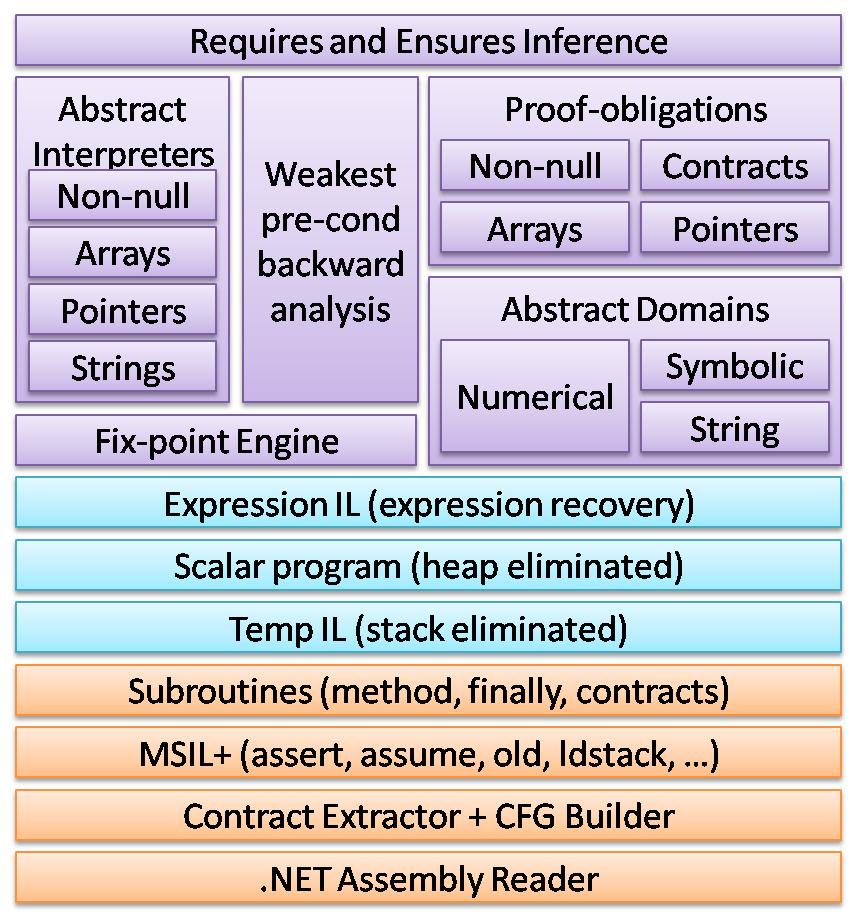
\includegraphics[scale=.5]{Architecture.png}
\caption{The \Clousot{} architecture.}
\label{fig:architecture}
\end{figure}




\section{Clousot}
We have implemented the abstract domain \Pentagons{} in our analyzer for .NET assemblies, \Clousot. 
\Clousot\ is part of the Code Contracts tools~\cite{CodeContracts}.
Code Contracts provide a language-agnostic way to express coding assumptions in .NET programs.
The contracts take the form of preconditions, postconditions, and object invariants. 
\Clousot\ checks each method in isolation, by assuming the precondition and asserting the postcondition.

The detailed structure of the analyzer is given in Figure~\ref{fig:architecture}.
\Clousot\ directly analyzes assemblies as produced by different .NET compilers as \code{csc} (for C\#), \code{vbc} (for VB), \code{fsc} (for F\#), etc.
At the bottom of the stack are the code providers, which provide a
low-level and stack-based, view of the code.  \Clousot{} has a
pluggable architecture that allows for different code providers and
contract providers.  For instance, one code provider can read
assemblies from disk, another could be a compiler, providing the code
being compiled directly.

The basic code fragment used is a \emph{subroutine}. We use subroutines to
represent several different aspects of code, such as fault/finally
handlers, pre- and post-conditions, and the normal method bodies. These
snippets are composed to form a complete control flow
graph. This approach makes it easy, for example, to form inheritance
chains for object invariants and postconditions, as well as sharing
precondition subroutines from all call-sites.

The higher abstraction levels take care of presenting a uniform view of the
code for specific analyses. They take care of
(i) injecting contracts as \code{assume}/ \code{assert} instructions;
(ii) removing the evaluation stack; (iii) abstracting the heap; and, (iv)
reconstructing the expressions that were lost by compilation~\cite{LogozzoMaf08-2}.

The value analyses at the top of the stack \emph{view} the code as a
normalized scalar program (similar to SSA form), where all the heap accesses have been
resolved and the contracts have been turned into a series of
\code{assume} and \code{assert} statements.  In particular, when
analyzing a public method \code{m}, of a class \code{C}, the
precondition of \code{m} and the object invariant of \code{C} are
turned into assumptions at the entry point, and the postcondition and
the object invariant of \code{C} are injected as assertions at the
exit point of \code{m}.  When analyzing a method which invokes
\code{m}, the precondition of \code{m} is asserted at the program
point just before the call, and the postcondition is assumed just
after the call.

\begin{figure}[t]
\centering
\subfigure[Disjunctive assertion]
{
\begin{tabular}{l}
  \code{if\ (*) } \\
  \quad\code{x := -1;}\\
   \code{else}  \\
  \quad\code{x := 1;} \\ 
  \code{assert\ x < 0 || x > 0;}
\end{tabular}
\label{fig:exDis}
}
\qquad
\subfigure[Overflow checking]
{
\begin{tabular}{l}
\code{Caller()} \\
\quad   \code{return\ FreshArray(5);} \\
\\
\code{FreshArray(int\ l)}\\
\quad \code{return\ new\ int[l-2];} 
\end{tabular}
\label{fig:exPre}
}
\caption{Assertion checking and precondition propagation in
  \Clousot{}. In the first case, a local backward analysis is used to
  discharge the assertion in the two incoming paths. In the second case,
  the implicit proof obligation $\code{l \geq 2}$ of \code{NewArray}
  is propagated to the caller. 
}


\end{figure}

\Clousot{} has two main phases: Analysis and checking.
The analysis phase is a forward abstract interpretation instantiated
with a user-specified abstract domain.
The entry (abstract) state is propagated through the method body, and
loops are handled with usual fixpoint computation. 
In theory, \Clousot{} infers an invariant for each program point.
In practice, it stores only the invariants at the loop headers to save
memory.

In the checking phase, \Clousot{} collects the proof obligations and
tries to validate them.
There are two kinds of proof obligations: (i) implicit, as for
instance array bounds checking and non-null dereferences; and (ii)
explicits as preconditions, postconditions, and user-provided assertions.
If \Clousot{} cannot discharge a proof obligation, it iteratively refines the
inferred invariants re-analyzing the method with more precise abstract
domains, as \eg\ SubPolyhedra~\cite{LavironLogozzo09}.
If the iterative refinement fails, then the analyzer performs a local
backward analysis  trying to validate the assertion for all the
incoming paths. 
This is useful to prove disjunctive assertions.
For instance, in Figure~\ref{fig:exDis}, \Pentagons{} (as well as other
non-disjunctive abstract domains) cannot validate the assertion. 
However, it can be propagated backwards to the two branches of the
conditional, and then discharged in each of them.
If the backward analysis fails, \Clousot{} tries to push the proof
obligation to the callers of the method.
For instance, in Figure~\ref{fig:exPre}, the array creation induces an
implicit proof obligation $\code{l \geq 2}$ which cannot be discharged
locally.
 \Clousot{} propagates it to the callers and checks it at the call sites (in the example
 $\code{5 \leq 2}$ trivially holds).
If none of the checking above succeed, then \Clousot{} reports a
warning to the user.

\section{Experimental Results}
\label{sec:experience}
\begin{figure}[t]
\centering
\small
\begin{tabular}{@{}r r |r r r| r r r  @{}}
         &  Bounds              & \multicolumn{3}{c|}{\Intervals} & \multicolumn{3}{c}{$\Intervals \times \SUB$}        \\
Assembly & checked & Valid & \% & Time & Valid & \% & Time     \vspace{3pt}  \\

\hline
\code{mscorlib.dll}      & 17 181 & 12 538 & 72.98 & 3:38 & 14 263 & 83.02 & 3:03  \\
\code{System.dll}        & 11 891 &  9 574 & 80.51 & 3:01 & 10 319 & 86.78 & 2:28  \\
\code{System.Web.dll}    & 14 165 & 12 350 & 87.19 & 3:39 & 13 030 & 91.99 & 2:49  \\
\code{System.Design.dll} & 10 519 &  9 322 & 88.62 & 2:56 & 10 132 & 96.32 & 2:18  \\
\hline
Average                  &        &        & 81.45 &      &        & 88.82 &       \\
\end{tabular}
\caption{The experimental results of the analyzer instantiated with Intervals alone, and with Intervals combined with Strict inequalities.}
\label{tab:results1}
\end{figure}


We present the experimental results of instantiating \Clousot{} with
\Pentagons{}. 
For arrays, \Clousot{} tries to validate that (i) the expression for a
\code{newarr} instruction is non-negative, and (ii) the 
index for the  \code{ldelem}, \code{stelem}, and \code{ldelema}
instructions is greater than or equal to zero and strictly smaller
than the length of the array. 

 
Figure~\ref{tab:results1},~\ref{tab:results2} and ~\ref{tab:results3} summarize the results of running the analysis on a subset of the .NET framework assemblies. 
 The analyzed assemblies are taken from the directory \code{\%WINDIR\% \backslash \allowbreak Microsoft\allowbreak \backslash} \code{Framework\backslash\allowbreak
  v\allowbreak2.0.\allowbreak50727} of  our laptop without modification or preprocessing.
The annotation of the framework libraries is ongoing~\cite{CodeContracts}. 
To provide an uniform test bench, we turned off the inter-method
capabilities of \Clousot.
All experiments were conducted on a Centrino 2 duo processor at 2.16 GHz, with 4 GB of RAM, running Windows Vista.

We ran the analysis with five different domains: \Intervals{} alone and the Cartesian product
\Intervals$\times$\SUB{} (Figure~\ref{tab:results1}); 
 \Pentagons{} without and with  constraint closure (Figure~\ref{tab:results2}); and \Octagons{}  (Figure~\ref{tab:results3}). 
We set a time out of 2 minutes per method.
In order to provide an uniform test bench, we switched off the
backward analysis and the precondition inference. 

The results show that with \Pentagons{}, \Clousot{} is able to validate on average 88.9\% of all array accesses in a little bit more than 3 minutes for the analyzed .NET assemblies.
As for the memory footprint, the analyzer never exceeded 300 Mbytes of RAM.

\subsection{Pentagons and non relational domains}

\begin{figure}[t]
\centering
\small
\begin{tabular}{@{}r |r r r| r r r r@{}}
                       & \multicolumn{3}{c|}{\Pentagons{} $\pjoin$} &  \multicolumn{4}{c}{\Pentagons{} $\pjoin^*$}  \\
Assembly &  Valid & \% & Time & Valid & \% & Time  & Timeout \vspace{3pt}  \\

\hline
\code{mscorlib.dll}       & 14 293 & 83.19 & 3:10 & 14 220 & 82.77 & 10:33 & 1 \\
\code{System.dll}         & 10 321 & 86.80 & 2:36 & 10 143 & 85.30 &  9:43 & 1 \\
\code{System.Web.dll}     & 13 034 & 92.02 & 2:55 & 13 048 & 92.11 &  8:30 & 0 \\
\code{System.Design.dll}  & 10 135 & 96.35 & 2:21 &  9 947 & 94.56 &  7:39 & 1 \\
\hline
Average                  &        & 88.89 &      &        &  88.10&       & 3\\
\end{tabular}
\caption{The experimental results of the analyzer instantiated with Pentagons and two different joins.}
\label{tab:results2}
\end{figure}

Figure~\ref{tab:results1} shows that combining \Intervals{} with symbolic upper bounds validates on average almost  10\% more array accesses than \Intervals{} alone for  a modest extra cost. 
\Pentagons{} without closure validate 78 extra accesses.
\Pentagons{} with closure produces almost no extra precision but the analysis time sensibly increases.
The analysis of three methods was aborted because it reached the 2 minutes timeout.
We manually inspected those  methods.
They turned out to be long methods (more than 1 300 instructions) with  complex control flow graphs using many distinct integer constants. 
Constants are captured by the numerical component of \Pentagons.
At join points, the closure step of $\pjoin^*$ materialized a quadratic number of new symbolic constraints which caused the slow down.

\subsection{Pentagons and Octagons}

Figure~\ref{tab:results3} presents the running times of Clousot instantiated with Octagons.
Our implementation of \Octagons{} uses sharing and sparse arrays to optimize performances.
Octagons caused an explosion of the analysis time: 35 methods timed out.
A larger timeout did not helped.
We inspected some of those methods. 
Once again, the problem is related to the propagation of numerical constants.
For instance, if $\code{b} = 1$ and $\code{y} = 2$, then the closure operation on \Octagons{} deduces the constraints $\code{b} - \code{y} \leq -1$, $\code{b} + \code{y} \leq 3$, $-\code{b} -\code{y} \leq -3$ and $-\code{b} +\code{y} \leq 1$.
However, if \code{b} and \code{y} correspond in the source code respectively to a \code{bool} variable and \code{int} variable  (Boolean are compiled to integers) then those constraints are meaningless.
It turns out that octagon constraints may relate too many \emph{logically} unrelated variables.
This behavior has already been observed by Min\'e ~\cite{Mine04} and Venet ~\cite{Venet04}, who proposed a solution based on the use of buckets.
The main idea behind buckets is to decompose an octagon of $n$ variables into a set of $k$ smaller octagons (buckets) each one with at most $n/k$ variables (typically four). 
Buckets may share some variables (pivots). 

In our setting, \ie{}   the analysis of MSIL, it is not clear how to partition variables into buckets or how to select the pivots.
Syntactic scope-based approaches do not work: in MSIL nested scopes inside methods are flatten.
Semantic based approaches as some form of backward analysis or type inference may be as expensive as the analysis with \Pentagons{} itself.

Pentagons are not a replacement for \Octagons{}. Octagons can validate
array accesses which are out of the scope of \Pentagons{}, for
instance because they involve the relation between two variables and a
numerical offset. 
We manually inspected the analysis logs for \code{mscorlib.dll}.
Octagons can validate 177 more array accesses than Pentagons. 
To increase precision, \Clousot{} allows a combination of \Pentagons{} and
\Octagons{} where constants are represented \emph{only} in
\Pentagons{} and \Octagons{} \emph{only} tracks  symbolic relations
involving \emph{exactly} two variables, that is constraints in the
form $\code{x} - \code{y} \leq k$ or $\code{x} + \code{y} \leq k$. 

In general we found \Octagons{} not to be a good compromise for \Clousot.
On one hand, the cost to validate implicit proof obligation as
array accesses with \Octagons{} is too elevated to be used in a build
environment.
On the other hand, \Octagons{} are not expressive enough to  support 
assume/guarantee reasoning.
In our experience, while most (numerical) preconditions
have the shape of Octagonal constraints (\eg $\code{x - y} < k$),
proving that they are established at the call site it requires a
relatively complex reasoning that often involves more than just
variables (\eg. Figure 1 of~\cite{LavironLogozzo09}). 
\Pentagons{} provide a better compromise than \Octagons{} in the managed
contracts setting.
They allow to quickly discharge ``easy'' proof obligations, and to  leave
the more complex ones to more expressive yet expensive abstract
domains as SubPolyhedra.




\begin{figure}[t]
\centering
\small
\begin{tabular}{@{}r  |r r @{}}
  & \multicolumn{2}{c}{\Octagons{} }  \\
Assembly &   Time & Timeout   \vspace{3pt}  \\
\hline
\code{mscorlib.dll}        &         1:38:43 & 20 \\
\code{System.dll}           &         1:09:00 & 13 \\
\code{System.Web.dll}       &         21:49 & 1 \\
\code{System.Design.dll}   &         17:44 & 1 \\
\hline 
& & 35
\end{tabular}
\caption{The execution times of the analyzer instantiated with Octagons}
\label{tab:results3}
\end{figure}


\section{Related work}
Early works on numerical abstract domains focused on program optimization.
Kildall described constant propagation in ~\cite{Kildall73}, the first example of a numerical abstract domain.
Karr refined constant propagation  using  linear \emph{equalities}~\cite{Karr76}. 
Cousot and Cousot ~\cite{CousotCousot77} introduced \Intervals{} as an example of abstract interpretation applied to  bounds checking elimination.

Cousot and Halbwachs noticed that numerical abstract domain can be used for program verification ~\cite{CousotHalbwachs78}.
They used Polyhedra, a numerical abstract domain to infer linear \emph{inequalities}, \ie\ constraints in the form $a_1\cdot \code{x}_1 + a_2\cdot \code{x}_2 \dots a_n \code{x}_n \cdot \leq k$.
Polyhedra are very powerful: they can be used for bounds checking, integer overflow detection, timing analysis, alias analysis, etc.
On the other hand, they encounter serious scalability issues~\cite{HalbwachsEtAl06}. 
Later research focused on optimizing Polyhedra.

The model checking and the constraint programming communities developed Difference bounds matrices (DBM) to handle constraints in the form $\code{x} -\code{y} \leq k$ or $\code{x} \leq k$. 
DBM are used to model-check timed automata~\cite{AlurDill90,ModelChecking} or answer queries~\cite{Revesz07}.
Min\'e extended DBM to fully-featured abstract domain (\Octagons,~\cite{Mine01-1,Mine01-2}) able to infer constraints in the form $\pm \code{x} \pm \code{y} \leq k$ in polynomial time.
A nice property of \Octagons{} is that the underlying implementation can be easily parallelized, \eg\ to exploit the power of modern graphics cards ~\cite{BanterleG07}.
Octagons have been generalized by Octahedra which capture linear constraints with \emph{unary} coefficients: $\pm \code{x}_1 \pm \code{x}_2 \dots \pm \code{x}_n \leq k$.  
Octahedra have an exponential worst case complexity which is reached in practice,~\cite{ClarisoCortadella07}.

Sankaranarayanan \emph{et al.} proved that a polynomial time algorithm for linear inequalities inference can be obtained  either (i) by fixing the number of linear equations \emph{before} the analysis~\cite{SankaranarayananEtAl05}, or (ii) by fixing a partial order between the variables in the program~\cite{SankaranarayananEtAl07}. 
In our setting, neither of the two hypotheses is realistic.

Laviron and Logozzo introduced SubPolyhedra~\cite{LavironLogozzo09}, which retain the same
expressive power of Polyhedra, but they give up some of the inference
power in order to achieve scalability.
SubPolyhedra precision can be finely tuned using hints.

Popeea \emph{et al.}~\cite{Popeea08} presented an interesting analysis to infer sufficient preconditions to eliminate bounds check inside method bodies. 
They underlying domain to their technique is Polyhedra. 
It would be interesting to see if faster results can be obtained using \Pentagons.


Xi and Pfenning~\cite{Xi98} presented a type checker to eliminate array bound checking in ML programs.
Courbot \emph{et al.}~\cite{courbot06} advocated the use of formal methods to optimize Java programs.
Unlike those two approaches, \Pentagons{} can synthesize loop invariants, hence presenting an higher level of automation.
 
Our analysis competes in performance with analyses developed to be used by the JIT, but it seems more precise: we got an average precision close to 89\% versus the 45\% reported in \cite{BodikEtAl00}.

Dor \emph{et al.} \cite{Dor03} use \Polyhedra\ and Allamigeon \emph{et al.} \cite{AllamigeonEtAl06} use \Intervals\ and a whole program
analysis to check overruns in string manipulation.  For the modular
nature of the code that we analyze we cannot perform a whole program
analysis, and the use of \Intervals\ without any symbolic reasoning on
upper bounds produces an analysis which is too imprecise (cf. Figure~\ref{tab:results1}).  
Larochelle \emph{et al.}~\cite{LarochelleEvans01} present an approach for buffer overrun checking similar to ours, using contracts and static checking.
However, their static analysis is limited by the syntax-oriented handling of loop invariants.



\section{Conclusions}
We presented a new numerical abstract domain, \Pentagons.  We
described its lattice operations, discussed its complexity and
presented an optimized algorithm for the join operator which runs in
(almost) linear time (instead of quadratic).

This abstract domain sits, as precision and cost are concerned, in
between the abstract domains of intervals and octagons.

We used \Pentagons{} to validate on average over 89\% of array
accesses in four major .NET assemblies in a couple of minutes. 
The remaining unproven accesses are discharge by using more precise, yet expensive domains on demand.

\textit{Acknowledgments.} We would like to thank the Anindya Banerjee, Corneliu Popeea, Pietro Ferrara and Vincent Laviron.

\bibliographystyle{plain}
\bibliography{bib}


\end{document}
